\documentclass[acmtog,anonymous,review]{acmart}
\acmSubmissionID{1234}

\usepackage{booktabs} % For formal tables

% TOG prefers author-name bib system with square brackets
\citestyle{acmauthoryear}
%\setcitestyle{nosort,square} % nosort to allow for manual chronological ordering



\usepackage[ruled]{algorithm2e} % For algorithms
\renewcommand{\algorithmcfname}{ALGORITHM}
\SetAlFnt{\small}
\SetAlCapFnt{\small}
\SetAlCapNameFnt{\small}
\SetAlCapHSkip{0pt}

% Metadata Information
\acmJournal{TOG}
%\acmVolume{38}
%\acmNumber{4}
%\acmArticle{39}
%\acmYear{2019}
%\acmMonth{7}

% Copyright
%\setcopyright{acmcopyright}
%\setcopyright{acmlicensed}
%\setcopyright{rightsretained}
%\setcopyright{usgov}
%\setcopyright{usgovmixed}
%\setcopyright{cagov}
%\setcopyright{cagovmixed}

% DOI
%\acmDOI{0000001.0000001_2}

% Paper history
%\received{February 2007}
%\received{March 2009}
%\received[final version]{June 2009}
%\received[accepted]{July 2009}

% !TEX root =  ShapeSpaceDog.tex

\usepackage{amsmath}
\usepackage{amssymb}
\usepackage{amsfonts}
\usepackage{enumitem}
\usepackage[mathscr]{eucal}
%\usepackage[ruled,vlined]{algorithm2e}
\usepackage{algorithmic}
\usepackage{microtype}
\usepackage{units}


% compact bullet lists and enumeration environments
\newenvironment{tight_enumerate}{
\begin{enumerate}[topsep=4pt,itemindent=\parindent]
  \setlength{\itemsep}{1pt}
  \setlength{\parskip}{0pt}
  \setlength{\parsep}{0pt}
}{\end{enumerate}}

%\newenvironment{tight_itemize}{
%\begin{itemize}[topsep=4pt]
%  \setlength{\itemsep}{1pt}
%  \setlength{\parskip}{0pt}
%  \setlength{\parsep}{0pt}
%}{\end{itemize}}


\usepackage{dsfont}
\usepackage{graphicx,wrapfig}

\usepackage{mdframed}
\mdfsetup{skipabove=\topskip,skipbelow=\topskip}
\newmdenv[	linewidth=0.75pt,
			leftline=false,
			rightline=false,
   			innerleftmargin=0pt,
			innerrightmargin=0pt]{topbot}

%\usepackage[mathcal]{euscript}

%\usepackage{amsthm}
%\newtheorem{theorem}{Theorem}[section]
%\newtheorem{lemma}[theorem]{Lemma}
%\newtheorem{proposition}[theorem]{Proposition}
%\newtheorem{corollary}{Corollary}
\newtheorem{mydefinition}{Definition}

\newcommand{\MiR}[1]{{\bf\textcolor{cyan}{MR: #1}}} % Michael
\newcommand{\OSH}[1]{{\bf\textcolor{red}{OSH: #1}}} % Olga
\newcommand{\TimH}[1]{{\bf\textcolor{blue}{TH: #1}}} % Tim 
\newcommand{\Rev}[1]{{#1}} % Revision

\newcommand{\todo}[1]{{\bf\textcolor{red}{TODO: #1}}}

%\newcommand{\newt}[1]{{\textcolor{blue}{#1}}}
\newcommand{\newt}[1]{{#1}}


%Abbreviations
\newcommand{\figref}[1]{Fig.\ \ref{#1}}
\newcommand{\secref}[1]{Sec.\ \ref{#1}}
\newcommand{\appref}[1]{Appendix \ref{#1}}
\newcommand{\equref}[1]{Eq.\ \eqref{#1}}
\newcommand{\defref}[1]{Def.\ \ref{#1}}
\newcommand{\lemmaref}[1]{Lemma \ref{#1}}
\newcommand{\theoremref}[1]{Theorem \ref{#1}}
\newcommand{\corollaryref}[1]{Cor.\ \ref{#1}}


% operators
\DeclareMathOperator*{\argmin}{arg\,min}
\DeclareMathOperator*{\argmax}{arg\,max}
\DeclareMathOperator*{\Proj}{Proj}


% Olga SH notation
\newcommand{\set}[1]{\mathcal{#1}}
% Transpose symbol
\newcommand{\transposeSign}{\textsf{T}}
\newcommand{\tr}{\transposeSign}


\newcommand{\R}{\mathds{R}}
\newcommand{\Z}{\mathds{Z}}
\DeclareMathOperator{\atantwo}{atan2}

\newcommand{\x}{x}
\newcommand{\p}{p}

\newcommand{\Fbo}{F_{\bar{1}}}
\newcommand{\Fbt}{F_{\bar{2}}}

\newcommand{\FAll}{\mathbf{F}}
\newcommand{\II}{I\!I}
\newcommand{\Atotal}{\mathcal{A}}


%\renewcommand{\ra}{\rightarrow}
\newcommand{\norm}[1]{\left\Vert#1\right\Vert}
\newcommand{\Norm}[1]{\lvert \! \lvert \! \lvert #1 \rvert \! \rvert \! \rvert}
\newcommand{\abs}[1]{\left\vert#1\right\vert}
\newcommand{\babs}[1]{\Big \vert#1 \Big \vert}
\newcommand{\bra}[1]{\left\{#1\right\}}
\newcommand{\parr}[1]{\left (#1\right )}
\newcommand{\brac}[1]{\left [#1\right ]}
\newcommand{\ip}[1]{\left \langle #1 \right \rangle }
\newcommand{\eps}{\varepsilon}


\newcommand{\alter}[1]{\textcolor{magenta}{[Alt: #1]}}
\newcommand{\opt}[1]{\textcolor{magenta}{[Opt: #1]}}
\newcommand{\rem}[1]{\textcolor{magenta}{[Rem: #1]}}

\newcommand{\LP}{\mathbb{L}}
\newcommand{\J}{\mathbf{J}}
\newcommand{\K}{\mathbf{K}}
\newcommand{\D}{\mathscr{D}}
\newcommand{\GR}{{\mathcal{G}}}
\newcommand{\I}{{\mathcal{I}}}
\newcommand{\CO}{\mathcal{C}}
\newcommand{\GI}{{\GR}_{\I}}
\newcommand{\GC}{{\GR}_{\CO}}
\newcommand{\M}{\mathcal{M}}
\newcommand{\Mevo}{{\M}_{evo}}
\newcommand{\Mgen}{{\M}_{G}}
%\newcommand{\u}{\mathscr{u}}
%\newcommand{\v}{\mathscr{v}}
\newcommand{\TD}{\ensuremath{T_{F}\D}}
\newcommand{\ND}{\ensuremath{N_{V(t)}\D}}
% Document starts
\begin{document}
% Title portion
\title{Curved Folded Discrete Orthogonal Geodesic Nets}

% DO NOT ENTER AUTHOR INFORMATION FOR ANONYMOUS TECHNICAL PAPER SUBMISSIONS TO SIGGRAPH 2019!
%\author{Gang Zhou}
%\orcid{1234-5678-9012-3456}
%\affiliation{%
%  \institution{College of William and Mary}
%  \streetaddress{104 Jamestown Rd}
%  \city{Williamsburg}
%  \state{VA}
%  \postcode{23185}
%  \country{USA}}
%\email{gang_zhou@wm.edu}
%\author{Valerie B\'eranger}
%\affiliation{%
%  \institution{Inria Paris-Rocquencourt}
%  \city{Rocquencourt}
%  \country{France}
%}
%\email{beranger@inria.fr}
%\author{Aparna Patel}
%\affiliation{%
% \institution{Rajiv Gandhi University}
% \streetaddress{Rono-Hills}
% \city{Doimukh}
% \state{Arunachal Pradesh}
% \country{India}}
%\email{aprna_patel@rguhs.ac.in}
%\author{Huifen Chan}
%\affiliation{%
%  \institution{Tsinghua University}
%  \streetaddress{30 Shuangqing Rd}
%  \city{Haidian Qu}
%  \state{Beijing Shi}
%  \country{China}
%}
%\email{chan0345@tsinghua.edu.cn}
%\author{Ting Yan}
%\affiliation{%
%  \institution{Eaton Innovation Center}
%  \city{Prague}
%  \country{Czech Republic}}
%\email{yanting02@gmail.com}
%\author{Tian He}
%\affiliation{%
%  \institution{University of Virginia}
%  \department{School of Engineering}
%  \city{Charlottesville}
%  \state{VA}
%  \postcode{22903}
%  \country{USA}
%}
%\affiliation{%
%  \institution{University of Minnesota}
%  \country{USA}}
%\email{tinghe@uva.edu}
%\author{Chengdu Huang}
%\author{John A. Stankovic}
%\author{Tarek F. Abdelzaher}
%\affiliation{%
%  \institution{University of Virginia}
%  \department{School of Engineering}
%  \city{Charlottesville}
%  \state{VA}
%  \postcode{22903}
%  \country{USA}
%}

%\renewcommand\shortauthors{Zhou, G. et al}

\begin{abstract}
% !TEX root =  CurvedFoldedDogs.tex
We present a computational framework for interactive design and exploration of curved folded surfaces, which is typically done in a manual physical process. Our objective is to lay the foundations for the digitalization of curved folded surface design.
We base our approach on modeling the shapes using discrete orthogonal geodesic nets (DOGs) in a piecewise manner. DOGs are used to represent the smooth parts of the modeled shape, and we connect different DOGs along curves that represent the sharp creases and folds. 
%, based on piecewise discrete orthogonal geodesic nets (DOGs). 
Our main 
%apparatus 
contribution is a discrete binary characterization for folds between DOGs, accompanied by an algorithm to simultaneously fold creases and smoothly bend planar sheets. We complement our algorithm with essential building blocks for curved folding deformations: objectives to control dihedral angles and mountain-valley assignments. We apply our machinery in a curved folding editing system, thus building the first tool capable of modeling bending and folding of complicated crease patterns.

% and explore areas previously uncharted by computer simulations such as wallpaper curved folding, as well as dynamically adding, removing, and moving creases along a flattened pattern.
\end{abstract}


%
% The code below should be generated by the tool at
% http://dl.acm.org/ccs.cfm
% Please copy and paste the code instead of the example below.
%
\begin{CCSXML}
<ccs2012>
<concept>
<concept_id>10010147.10010371.10010396.10010397</concept_id>
<concept_desc>Computing methodologies~Mesh models</concept_desc>
<concept_significance>500</concept_significance>
</concept>
<concept>
<concept_id>10010147.10010371.10010396.10010398</concept_id>
<concept_desc>Computing methodologies~Mesh geometry models</concept_desc>
<concept_significance>500</concept_significance>
</concept>
</ccs2012>
\end{CCSXML}

\ccsdesc[500]{Computing methodologies~Mesh models}
\ccsdesc[500]{Computing methodologies~Mesh geometry models}

%
% End generated code
%


\keywords{curved folding, developable surfaces, discrete differential geometry, geodesic nets, shape modeling}



\maketitle
\section{Introduction}
There are myriads of ways to deform a planar sheet without stretching or tearing it. One can bend it, fold it, or combine the two. Folding and bending isometries are different by nature, and historically speaking there is some dichotomy in the study of the two; Smooth isometries are typically studied in differential geometry \cite{do_carmo}, whereas straight folds are often explored in the field of computational origami \cite{origami_book}. Curved folded surfaces \cite{huffman} results from a combination of the two, as folding an inextensible sheet along a curve necessitates global bending around the crease.

Building curved folded sculptures is a manual and time consuming process, often done using an empirical trial and error approach  as little theory is known \cite{curved_review,huffmann_reconstructing}. Contrary to classical origami, bending and folding instructions are hard to write down and the fact that multiple creases need to fold simultaneously further complicates the process \cite{StringActuated:2017}. In practice, artists often pre-crease the paper using a ball burnisher or a CNC plotter before carefully folding and bending it.

Albeit manual, slow, and exhaustive, playing with paper is currently the only option available for an explorer of curved folds. Existing works on modeling these surfaces are either limited to previously discovered sculptures \cite{curved_folding_kilian,StringActuated:2017} or model a small partial set of folded surfaces generated by reflections or rotational sweeps \cite{Mitani_ref,mitani2009design}. Modeling the folding process of novel forms remains a challenge \cite{curved_review}. In this paper we set to develop the basic tools for unconstrained modeling of curved folds, in order to aid the exploration, analysis and study of new curved folded structures.

Our work builds upon Discrete Orthogonal Geodesic Nets (DOGs) \cite{rabi18,rabi2018shape} as a discrete model for smooth developable surfaces parameterized by orthogonal geodesics. These are regular quadrilateral meshes with equal angles around each vertex, and unlike other computational models for developables do not suffer from locking of various deformation modes \cite{locking1,locking2,grin_shells}, are not fixed to predetermined rulings directions \cite{pottmann_new,curved_folding_kilian} or require remeshing while deforming the surface \cite{StringActuated:2017,SchreckEG2017,Narain}. We represent curved folded models as piecewise smooth developable surfaces with tangent discontinuities and equal geodesic curvature along their intersections, as done in \cite{rabi2018shape}. 

% Bifurcation mode... Explains that it doesn't have to fold, and it is more complicated when there are more folds, and hence one needs to give a simple definition and algorithm for folding. Then continue that there are other parameters one would like to control such as angles and rulings, and bla bla.
The challenge is then to find deformations that leads to a folded configuration (ADD:FIGURE).

% There are 2 components for such modeling. The first is a good model, the second is a way to navigate and fold that model, similarly as to how one needs to place is fingers in order to fold a piece of paper. We use the model


% The beautiful art of curved folded sculptures is almost a hundred years old, dating back to the 1920's works of Josef Albers in the Bauhaus art school \cite{josef_albers_thesis}, and continuing with the investigations of David Huffman and Ron Resch in the 1970's \cite{huffman,resch1974portfolio}. 

% Many of these early works, are mathematically not yet fully understood. We know what happens in one fold, but multiple ones still forms a challenge and we only have specific investigation for some cases. Creating them is , using paper and They date to 1920's but we only know what happen along one fold, or analyze specific set of examples, and don't know how typical models even fold. Computer simulations of that can help, but are somehow legging behind what is mostly experimented by hand, in a process that is in fact time consuming, often involving using a pen bla and da da da.

\section{Related work}
\subsection{Modeling developable surfaces}
A smooth surface is called a \textit{developable surface} if it is locally isometric to the plane, or equivalently has zero Gaussian curvature. Though well understood mathematically \cite{do_carmo,spivak,computational_line}, there is a plethora of work on modeling developable surfaces, which has been proven to be a challenge. The primary difficulty lies in using a discrete model that is able to capture the full set of deformations keeping a surface developable. These include extrinsic deformations as well as intrinsic deformations. The latter stretch a surface while keeping it developable, and is used for geometry exploration tasks where the size and shape of the flattened developable surface is unknown \cite{conical,pottmann_new,rabi2018shape}. A failure of a discrete model to discretize the full range of smooth deformations is often termed \textit{locking} \cite{solomon,locking1} and is the bane of most discrete developable models. Ruling based models \cite{conical,curved_folding_kilian,pottmann_new,stein_dev,solomon} are limiteds to a partial set of extrinsic deformations while isometry based methods \cite{grin_shells,shells, goldenthal2007efficient,froh_botsch} do not model intrinsic deformations by design, but are also prone to locking of various bending deformations \cite{locking1,locking2}, and are often coupled with dynamic remeshing \cite{narain2012adaptive,StringActuated:2017,Narain,SchreckEG2017}. \MiR{should I explicitly say that remeshing is complicated and is also not backed up by any theory?} Our work is based on modeling a developable surface as a discrete orthogonal geodesic net (DOG) \cite{rabi18}, a model that have been shown both theoretically and empirically to avoid extrinsic or intrinsic deformations locking. We further rely on \cite{rabi2018shape} to deform and explore the shape space of DOGs, but replace the authors' Laplacian flow deformation with an SQP algorithm as further detailed in \secref{sec:implementation}.
\subsection{Curved folding}
The beautiful art of curved folded sculptures is almost a hundred years old, dating back to the 1920's works of Josef Albers in the Bauhaus art school \cite{josef_albers_thesis}, and continuing with the investigations of David Huffman and Ron Resch in the 1970's \cite{huffman,resch1974portfolio}. This art, though intimately linked to the mathematics of developable surfaces, is mostly driven by physical experiments with paper \cite{curved_review}. As opposed to smooth developable surfaces \cite{do_carmo} or straight fold origami \cite{origami_book}, the mathematics of curved folding is legging behind the manual craft, and mostly concerns the local behavior of a single folded curved crease \cite{duncan_folded,mathematical_omnibus,curved_review}. Notable crease patterns such as the Huffmann Tower \cite{huffman2,huffmann_reconstructing}, are not yet understood \cite{demaine2018conic} and the known mathematics on folding and bending multiple curved creases is limited to a very few particular cases, coupled with a specific folding movement and guided by fixed rulings \cite{demaine_lens, demaine2018conic}. In essence, we do not know much about which crease patterns fold, and we do not know in which ways they can fold; Unlike straigh origami, there are often infinite ways of folding bending a curved crease pattern by varying the dihedral angles as well as the developable rulings along different creases. \\
Curved folding was first introduced to the geometry processing community by work of \cite{curved_folding_kilian}, who reconstructed scanned curved folded surfaces. In \cite{StringActuated:2017} the authors simplify the process of fabrication of curved folded models using a string actuation network. Both of these works assume an access to known target surfaces. Other works on modeling developable surfaces focus on a given subset of folds, such as planar creases generated by reflection \cite{mitani2012column,Mitani_ref}, surfaces generated by rotational sweeps \cite{mitani2009design}. The works \cite{pottmann_new} model curved folded surfaces with a rigid ruling pattern. We note that the majority of curved folding deformations change the rulings throughout the folding process. 
% Write that the only system of freeform exploration of curved folding that the authors know of is based on DOGs, that this hits a limit with multiple creases and that we extend upon that work (refer to fig 2 again).
\section{Setup} \label{sec:setup}
\subsection{Definitions}
Throughout the paper, we use the following definition for a curved folded surface:
\begin{definition} \label{def:curved_folded_surface}
A surface $S$ is called a curved folded surface if it is locally isometric to the plane and can be written as $S = \bigcup P_i $ where each $P_i$ is a $C^2$ developable surfaces termed a \textit{patch}, and their intersections $P_i \cap P_j$ are $C^2$ curves.
\end{definition}
% consists piecewise $C^2$ developable surface whose discontinuities are focused along $C^2$ curves. More formally, 
This definition is suitable for various topologies, such as a cylinder, although throughout the paper we will work with surfaces that can be globally isometrically flattened to the plane. Borrowing terms from \cite{origami_book,non_pleated}, we often refer to the surface \textit{crease pattern} consisting of the planar isometric surface domain $S_P$ together with the flattened intersection curves between the interior of the patches $P_i$ (see \figref{fig:crease_pattern}). The flattened domain boundaries together with the flattened intersection curves form a (pseudoline) planar arrangement \cite{arrangements}, inducing a planar graph decomposing $S_p$ into different disconnected components termed faces, which are domains isometric to the patches $P_i$. The vertices of this graph are the intersection of the curves with each other or the boundary curves, which we call \textit{crease vertices}. The \textit{edges} of this graph are curves isometric to the intersections of the various patches (see \figref{fig:crease_pattern}), and we refer to the inner points of these curves as \textit{crease points}, i.e. points on these curves that are not \textit{crease vertices}. We say that $S$ is \emph{folded} along a crease point if at this point the patches $P_i,P_j$ sharing it has a tangential discontinuity (see \figref{fig:folded_and_not_folded}).

\begin{figure} [h]
	\centering
	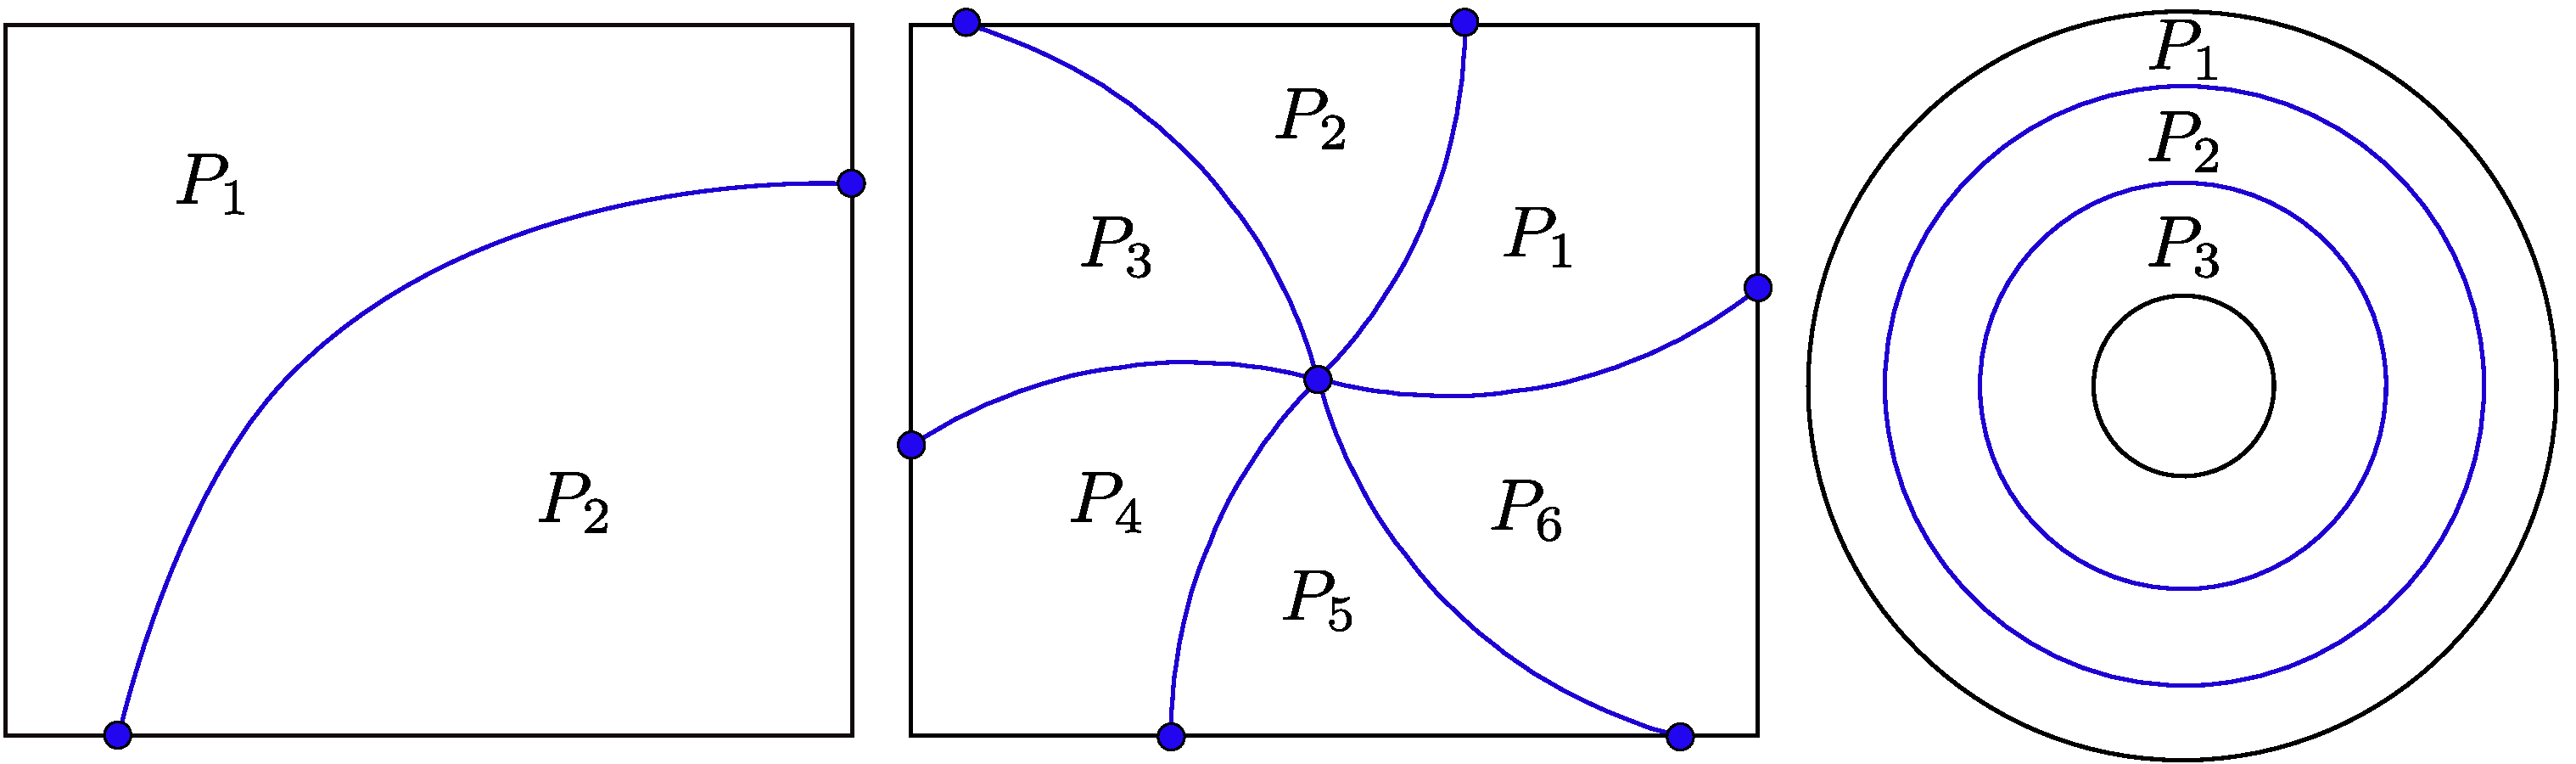
\includegraphics[width=\linewidth]{figures/crease_patterns}
	\caption{Curved crease patterns, decomposing a pattern into multiple components $P_i$ and intersecting at crease vertices. Boundary curves in black, crease curves in blue.}
	\label{fig:crease_pattern}
\end{figure}
We are interested in deformations on curved folded surfaces that keeps them curved folded. Viewed separately on each patch $P_i$, these deformation are $C^2$, though they often introduce tangent discontinuities along the patches intersections. At \cite{demaine_lens} the authors refer to creases that remain $C^2$ as \textit{smoothly folded} creases (though they define it as $C^1$ they prove that this implies that they are $C^2$). In particular we are interested in such continuous deformations, or deformation flows \cite{rabi2018shape}, which we refer to as curved folding flows. We denote these flows by a continuous map $S(t), 0 \leq t \leq 1$, where each $S(t)$ is a curved folded surface and the flow is $C^2$ when limited to each patch. We often look at the case where the starting point $S(0)$ planar. In this paper we focus on modeling isometric curved flows, which we also refer to as \emph{folding}. These flows can can be used to model physical paper or metal folding, though most of our observations and tools can also be used to model curved folding flows that are not isometries. Non-isometric developable deformations can be useful for design tasks where the a-priori flattened shape is unknown \cite{rabi18,rabi2018shape} .

\subsection{Model} \label{sec:model}
We follow the work of \cite{rabi2018shape} by modeling each patch $P_i$ as a discrete orthogonal geodesic net (see \figref{fig:curve_on_dog}). We represent a crease as piecewise linear curves, whose points $c(i)$ are represented by the curves' intersection point with the grid edges. Each point $c(i)$ is a linear combination of two vertices on a DOG: $c(i) = t v_i + (1-t)v_j,$ where $0 \leq t \leq 1$ and $v_i,v_j$ are too neighbour vertices on the grid.  Each point on a crease lies on each of the $m \geq 2$ different patches, essentially duplicated. If $c(i)^1,c(i)^2,....,c(i)^m$ are the representation of $c(i)$ on the different patches, we enforce constrain these duplicated points have equal coordinates (see \figref{fig:curve_on_dog}).
We trivially extend the represntation at \cite{rabi2018shape} to support intersecting curves by adding grid lines at crease vertices (see \figref{fig:piecewise_dog_from_crease} and \figref{fig:curve_on_dog}).

\begin{figure} [h]
	\centering
	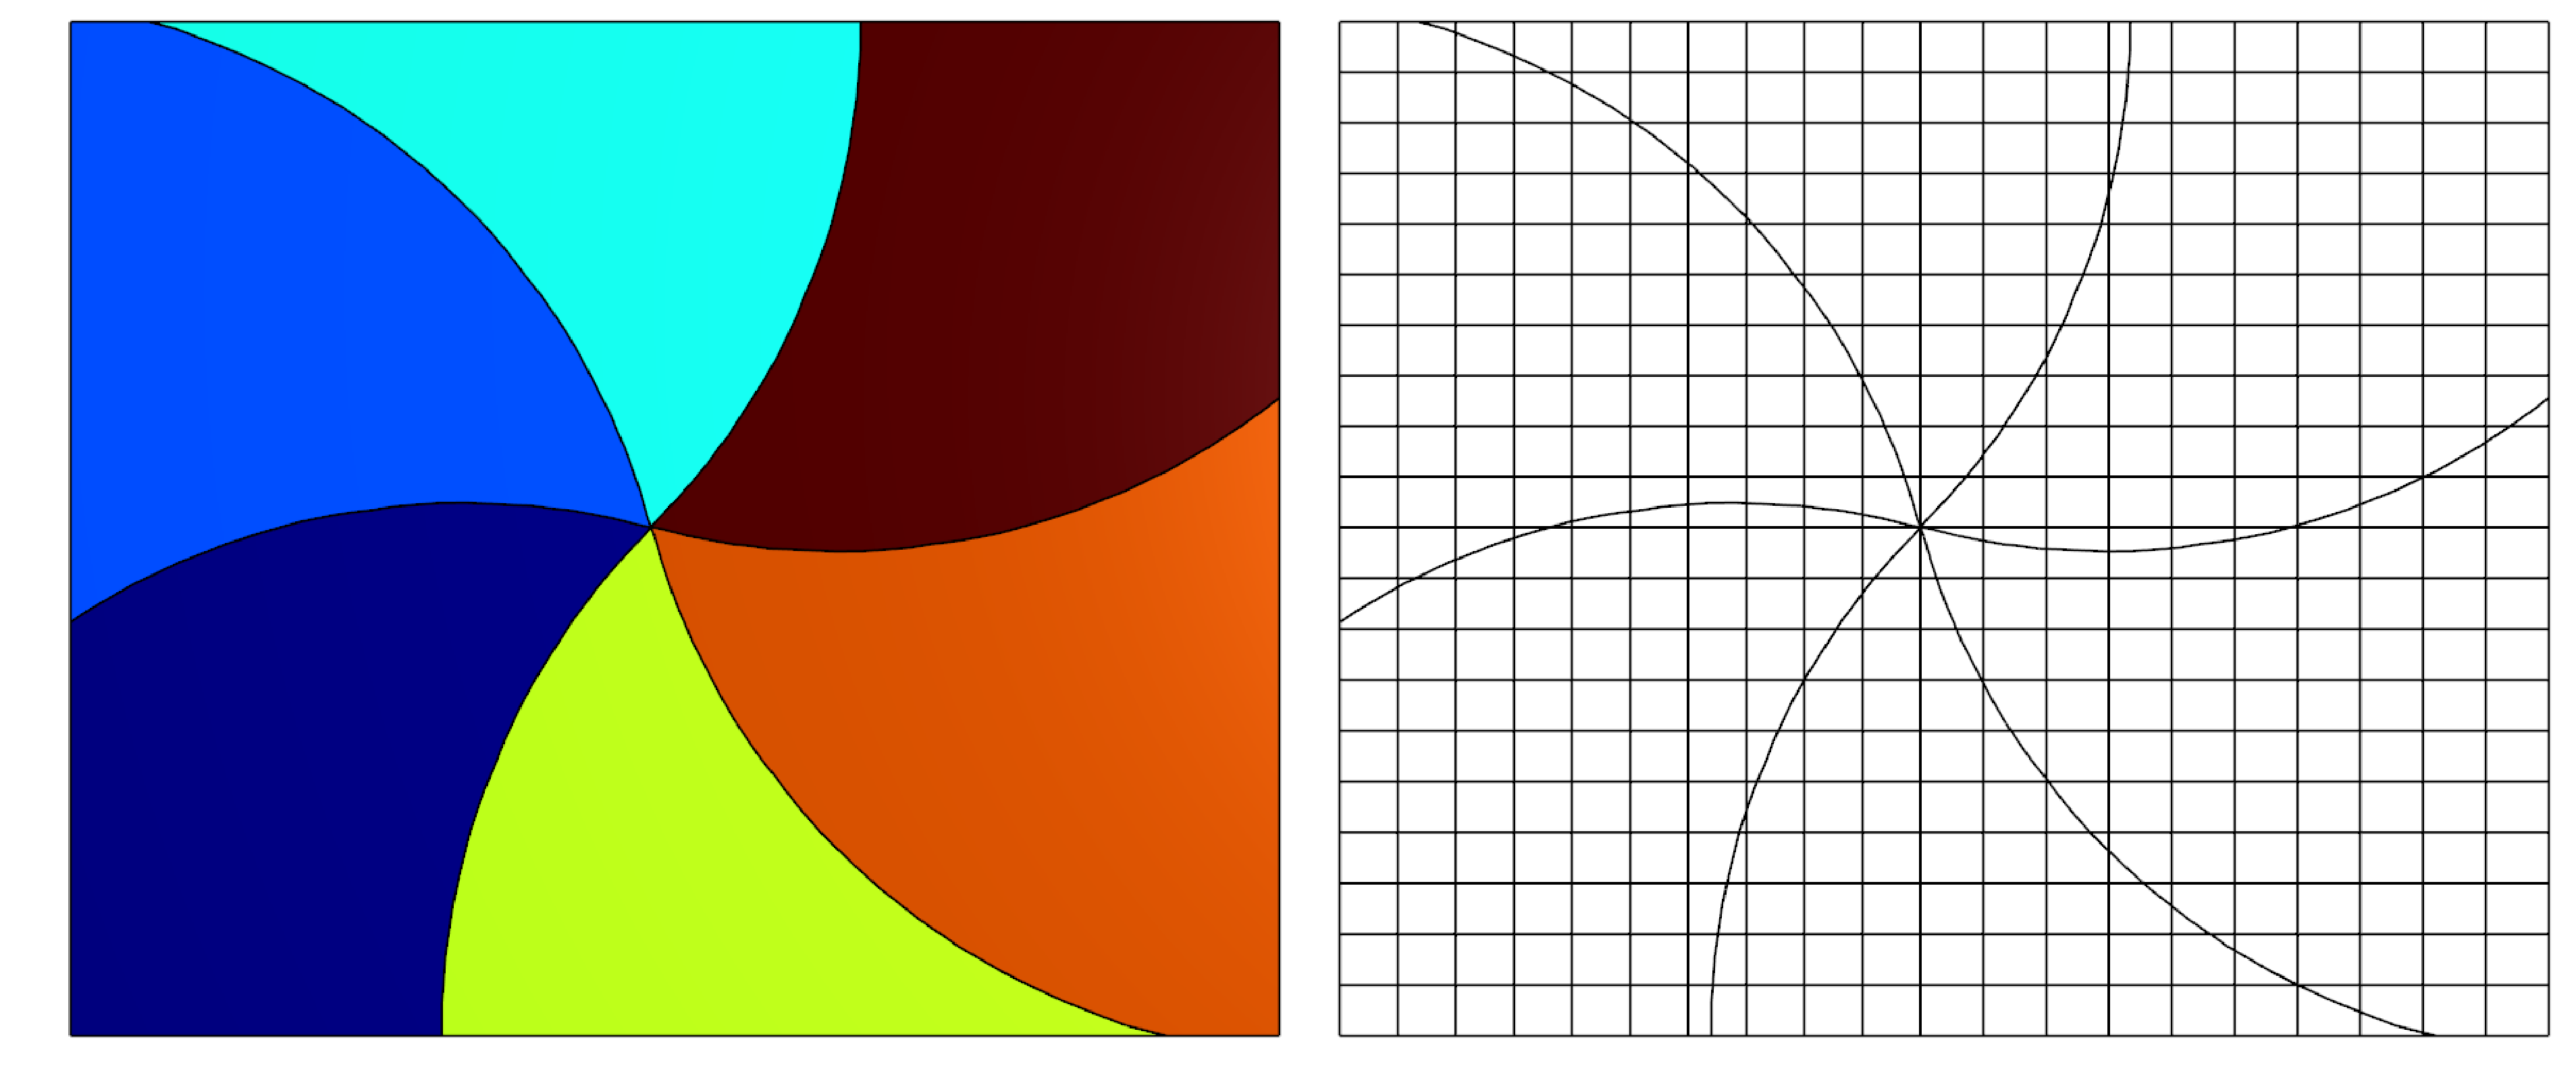
\includegraphics[width=0.8\linewidth]{figures/piecewise_dog_from_crease}
	\caption{Given a crease pattern, we create a DOG for each segment (colored differently), and use the boundary constraints as done in \cite{rabi2018shape}.}
	\label{fig:piecewise_dog_from_crease}
\end{figure}

\begin{figure} [h]
	\centering
	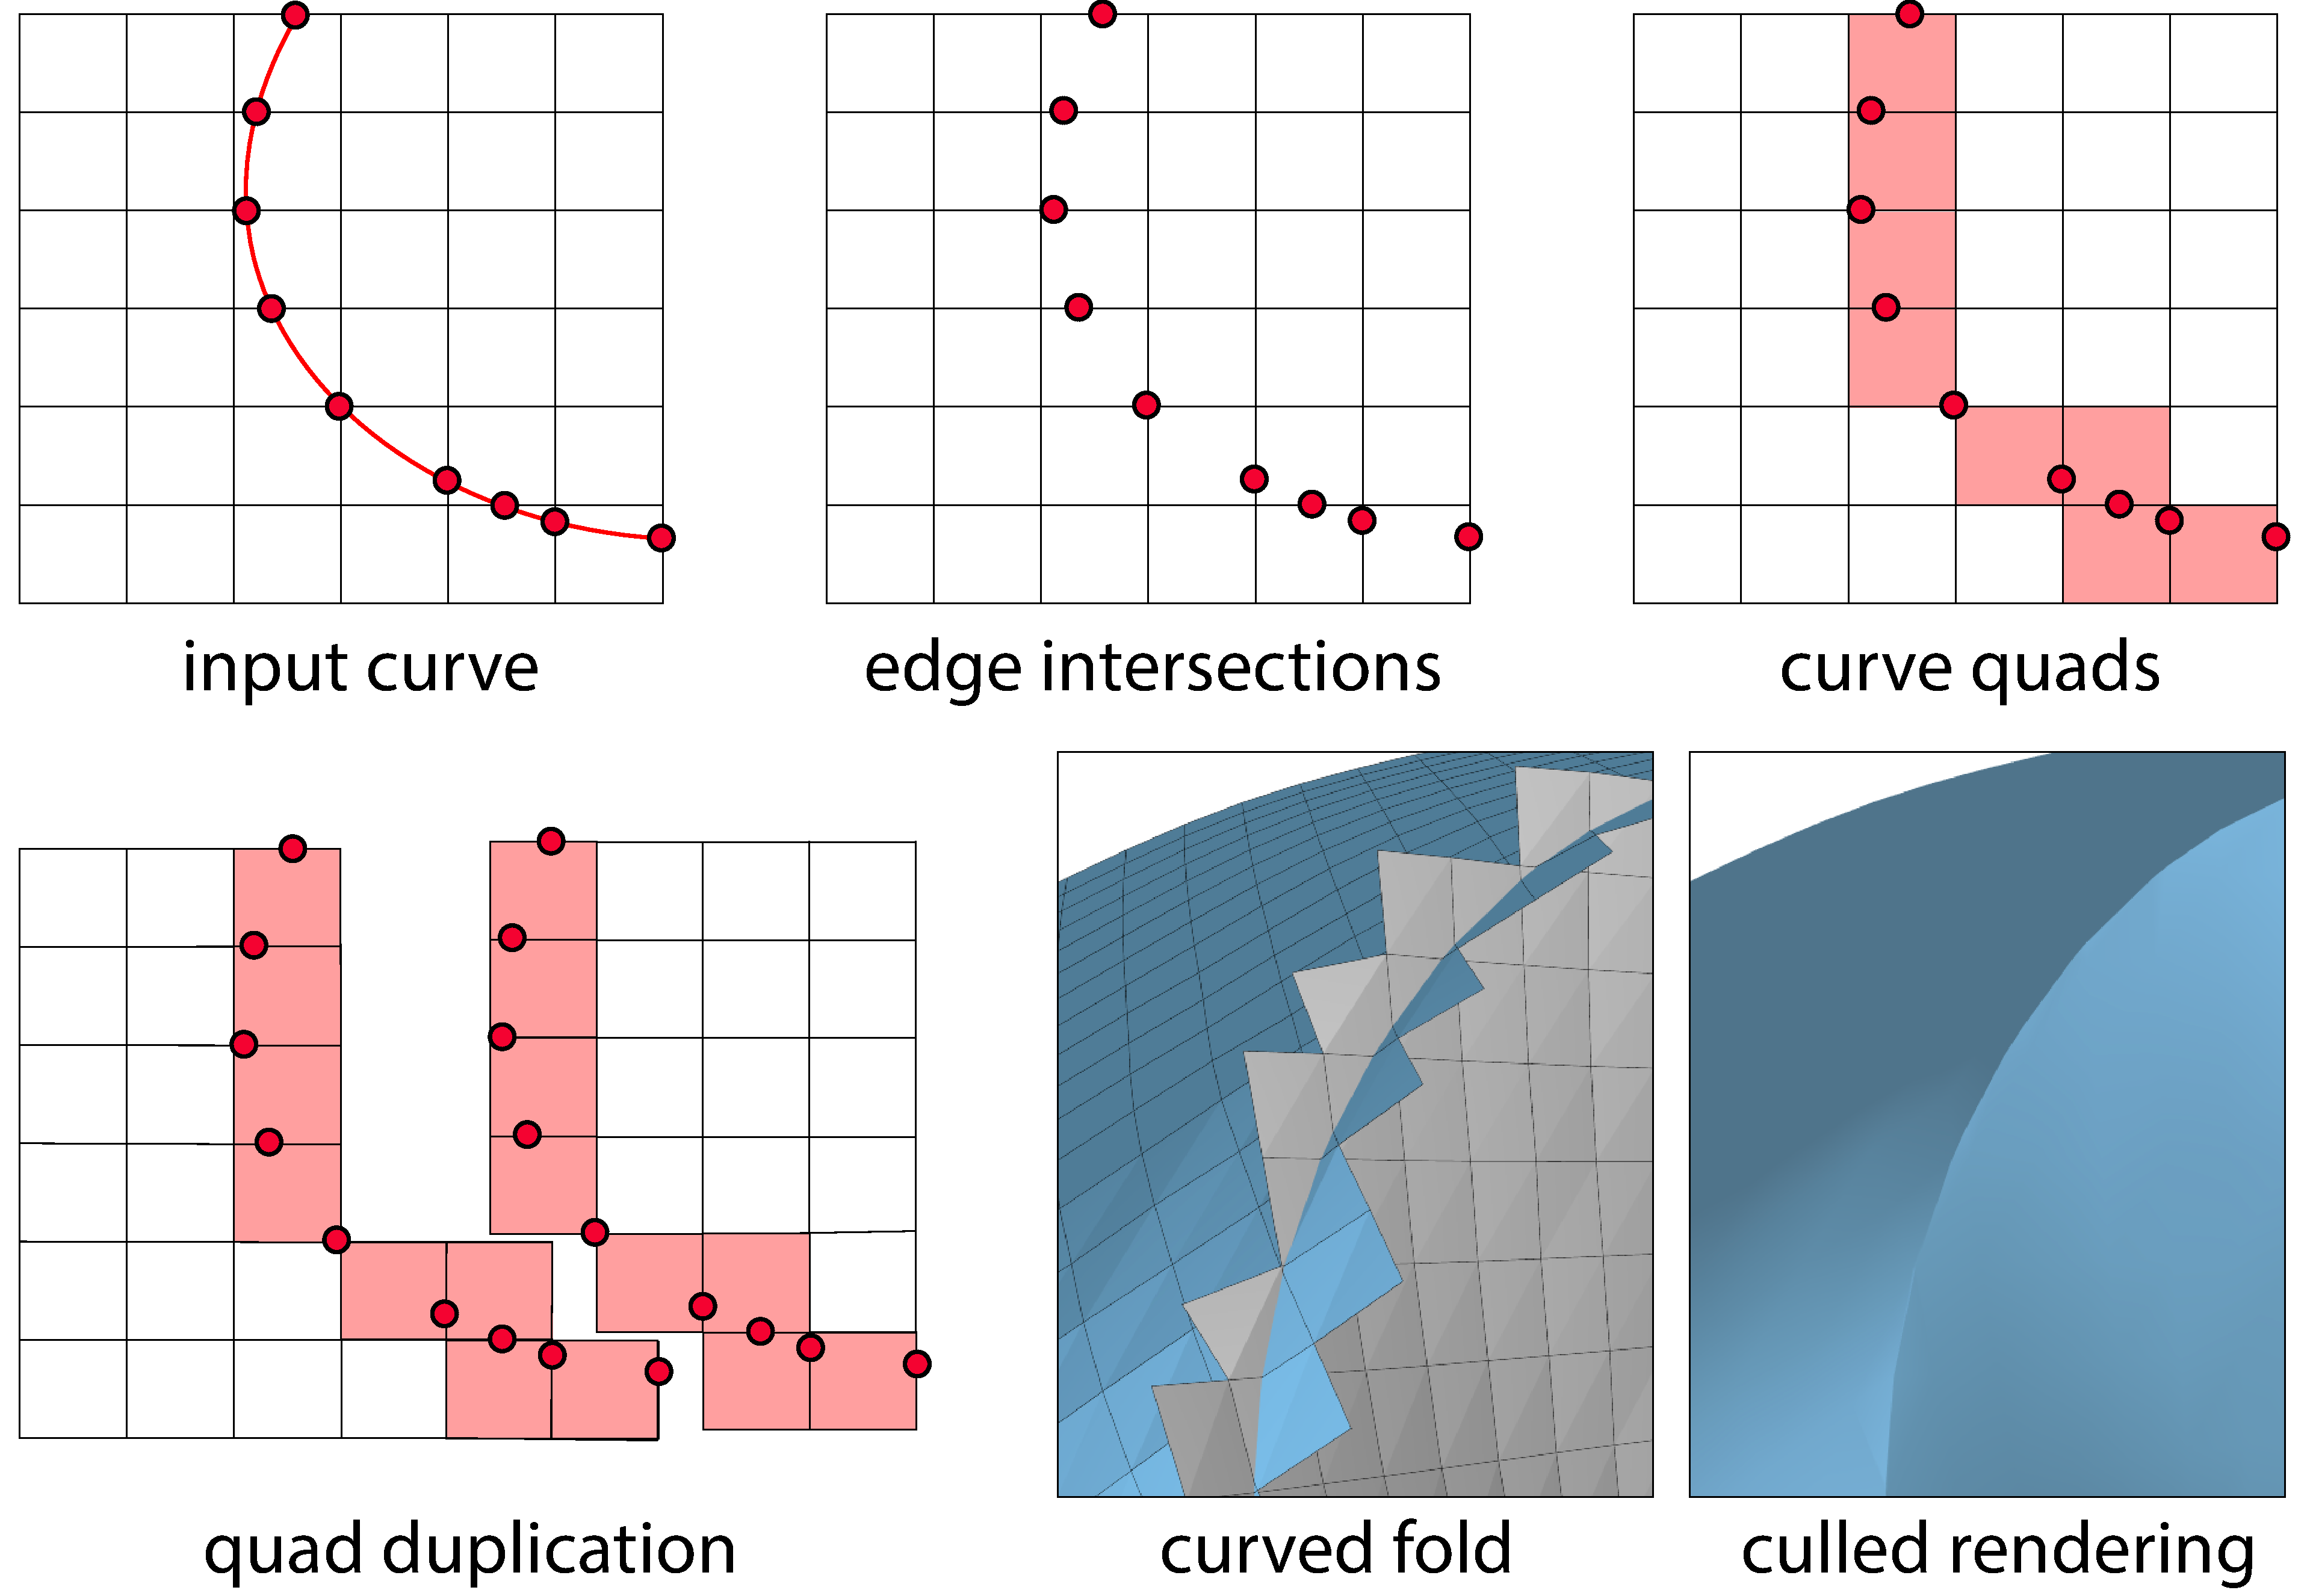
\includegraphics[width=0.8\linewidth]{figures/curve_on_dog}
	\caption{Picture taken from \cite{rabi2018shape}.}
	\label{fig:curve_on_dog}
\end{figure}

\subsection{Desiderata}
Our goal is to develop tools for the exploration of curved folded shapes on top of piecewise DOGs by means of deformations. Our choices are guided by the following ground rules for deforming DOGs:
\begin{enumerate}
  \item Perform homotopy based optimization \label{homotopy_opt}
  \item Minimally constrain DOGs \label{minimal_const}
%  \item Use accurate functionals \label{accurate_func}
%  \item Use simple functionals
\end{enumerate}
\textbf{Homotopy based optimization} is motivated both theoretically and empirically; Modeling DOGs requires solving highly constrained and non linear optimization problems, yet the theory of DOGs guarantees the existence of nearby solutions if one starts at a feasible point. In fact, generally the shape space of DOGs is a smooth manifold \cite{rabi2018shape}. This observation is worthwhile in practice; DOGs exploration was demonstrated to perform well using smooth flow, or homotopy based optimization methods both for handle based editing tasks as well for more complicated deformations such as curve-constraining flows \cite{rabi2018shape}. \\
\textbf{Minimally constrain DOGs.} As DOGs are already heavily constrained, one needs to carefully choose which quantities to constrain by hard constraints, and which ones should be optimized using soft constraints. This is essential to avoid locking, or ill-posed problems in case the constraint gradients are linearly independent \cite{rabi2018shape}. In particular, the rigidity analysis in \cite{rabi18} demonstrates that one cannot fix all edge length exactly, or likewise demand a DOG to also be a Chebyshev net. We note however that this can be done approximately and to a low tolerance as a DOG is a chebyshev at the smooth limit and at the smooth limit there is a rich set of exact isometries. The folding constraints at \secref{sec:folding} where chosen such that they could be satisfied \textit{exactly}, and so that in practice they vanish once the surface is sufficiently folded, just like a piecewise smooth curved folded surface. \\
%\textbf{Accurate functionals.} We look for constraints and objectives that are accurate and as often in the case with DOG objectives, converge under sampling of a smooth orthogonal geodesic net \cite{rabi18,rabi2018shape}. \\
%\textbf{Simple functionals.} We strongly prefer sparser objectives with a lower degree as possible. To that end, we leverage the regularity of the DOG meshing and theory on smooth orthogonal geodesic nets in our derivations. \\
\section{Fundamental tools for folding} \label{sec:folding}
In this section, we explore the different ways one can fold a given crease pattern, and derive objectives to control them.


\subsection{Curved folding from the view of the crease} \label{sec:curved_folding_from_a_curve}
Let $\Gamma(t)$ be a curve on a smooth developable surface $S$,  let $\gamma(t)$ be its flattened curve, $k(t)$ its curvature, and $k_g(t)$ its geodesic curvature such that $k_g(t) = k(t) \cos(\alpha(t))$ for some $\alpha \neq 0$. This implies that at each point along $\Gamma(t)$, the tangent planes of $S$ make an angle of $\alpha$ with the osculating planes of $\Gamma(t)$. One can switch this point of view: start with a flat curve $\gamma(t)$, isometrically embed the curve in $\mathbb{R}^3$ and construct a developable surface by reconstructing the planes at each point. As long as the crease is curved, i.e. has some normal curvature such that $k(t) > k_g(t)$ and $\alpha(t) \neq 0$ then there are 2 distinct planes containing $\Gamma'(t)$ and forming an angle of $\alpha(t)$ with the curve's osculating plane. Therefore, one can locally construct two different smooth developable surfaces passing through $\Gamma(t)$ with $\gamma(t)$ as its flattening. Alternatively, one can construct a folded surface by a consistent smooth choice of a different tangent plane for each "side" of the curve (see Fig. \ref{fig:curved_fold_through_curve}) \cite{more_on_paper}. The tangent planes from both sides are reflections of one another through the osculating plane of the curve \cite{curved_folding_kilian}.

\begin{figure} [h]
	\centering
	\includegraphics[width=0.7\linewidth]{figures/curved_fold_through_curve.pdf}
	\caption{(TODO BETTER FIG) Left: A flattened curve in 2D. Right: A small neighbourhood around an embedding of the curve in $\mathbb{R}^3$, its osculating plane and two options to extend a the curve to developable surface by constructing the 2 planes containing the curve's tangent and making an angle of $\alpha(t)$  with the osculating plane. Choosing 2 different tangents along each 'side' of the curve creates discontinuities along the curve and a curved folded surface.}
	\label{fig:curved_fold_through_curve}
\end{figure}

%Two intersecting developable surfaces can be flattened along their intersection if the intersected curve have the same geodesic curvature on both surfaces. 
\subsection{The smooth and combinatorial parameters of a single crease}
A single straight crease is rather boring, mathematically speaking. Straight lines can only be folded as in classical origami, i.e. by keeping them straight \cite{demaine_lens}. Hence the folding process of a single fold can be described by a single real number, representing the fold dihedral angle. As detailed in section \secref{sec:curved_folding_from_a_curve}, there are far more degrees of freedom for folding a curved crease; Up to rigid motion, this folding could be described by two smooth \textit{functions}: the curves' curvature $k(t) \geq k_g(t)$ and its torsion $\tau(t)$. Unlike the case of classical origami, the folding angle of a curved crease can vary along the curve. The folded shape is locally not determined only by these two smooth functions as there is an additional \textit{combinatorial} degree of freedom: the choice of a surface at each side (see \figref{fig:curved_fold_through_curve}). There are four options, two of which creates creates discontinuity along the crease. We call one folded configuration a mountain fold and the other a valley fold. %We follow \cite{demaine_lens} to distinguish between the two type of folded configurations by calling one choice a \textit{Mountain} fold and the other a \textit{Valley} fold. %We note that by \cite{demaine_lens}, a fold always consistently stays mountain/valley throughout the entire creased curve. Assuming a given normal orientation, a fold is said to be a mountain fold if the normal of the surface TODO:ADD EXPLANATION. 


%The curvature and torsion also dictates the ruling patterns of the developable surfaces, generally changing while folding and bending the surface. Deforming a curved crease locally determines the shape of both surfaces around it, and the exact regions of surfaces influenced by that fold depend on the ruling patterns themselves. As mentioned, the rulings patterns themselves can change which can smoothly change during the deformation itself. 

%(there's the cone singularity case where a curved fold is more local (as focused on the cone point) but I think this requires the curve to be C^1.. should mention it?

\subsection{The combinatorial parameters of multiple creases}
Curved folding is well understood locally, around a small part of a single curve, as the tangent planes along the curves are reflections of one another through the folded curve osculating plane. Understanding crease patterns globally still remains a challenge. In essence, deforming one patch propagates a global deformation of the patch on the other side of the crease, a process that depends on the ruling patterns. The ruling patterns are formed as the intersections of the tangent planes, and as mentioned the ruling patterns can smoothly change during the deformation itself. When there are multiple creases this process further propagate and dictates the shape of other patches (see \figref{fig:multiple_crease_pattern}). The process becomes more complicated when some creases intersect due to compatibility constraints (see \figref{fig:multiple_crease_pattern}, right figure). Generally speaking, choosing the first mountain/valley assignment of one fold dictates the mountain/valley assignments of the other folds as the location of another creased is fixed (TODO: see if I can cite demaine-tachi or if that is still unpublished). The combinatorial degrees of freedom that then remain are to determine which folds are active, i.e. folded (TODO: see figurebias-stuff).

% Can change the sentence above to not talk about mountain or valley yet, if needed.
% The pictures which will show are then discrete, though the smooth picture is the same. Maybe put the discrete picture in the setup as well.
% A fold is active if nearby tangents are reflections of one another, and is not active if they are the same as there is no discontinuity. (have a figure that is discrete, but explain it is also the same drawing for the smooth case).
% Write down the formula. Write down a flow. State it is inequality hence folding should be done at time = 0 when it is flat, but nevertheless a binary decision. We characterize it by the sign. 
% One can then view a folding-bending process as a smooth flow, i.e. a smooth deformation on a piecewise C^2 developable surface. The choice to make each fold active is only done during time t = 0, whereas otherwise discontinuties arise, and locally remains a curved fold as the equality.
% Problem in using it for a DOG is that we cannot hope to get it exactly. Then present binary representation. Say how it's really good (also goes to zero very fast).
% The binary characterization in the smooth case, motivate more degrees of freedom, and add the algorithm. Then add control for dihedral angles and mountain valley fold.

\begin{figure} [h]
	\centering
	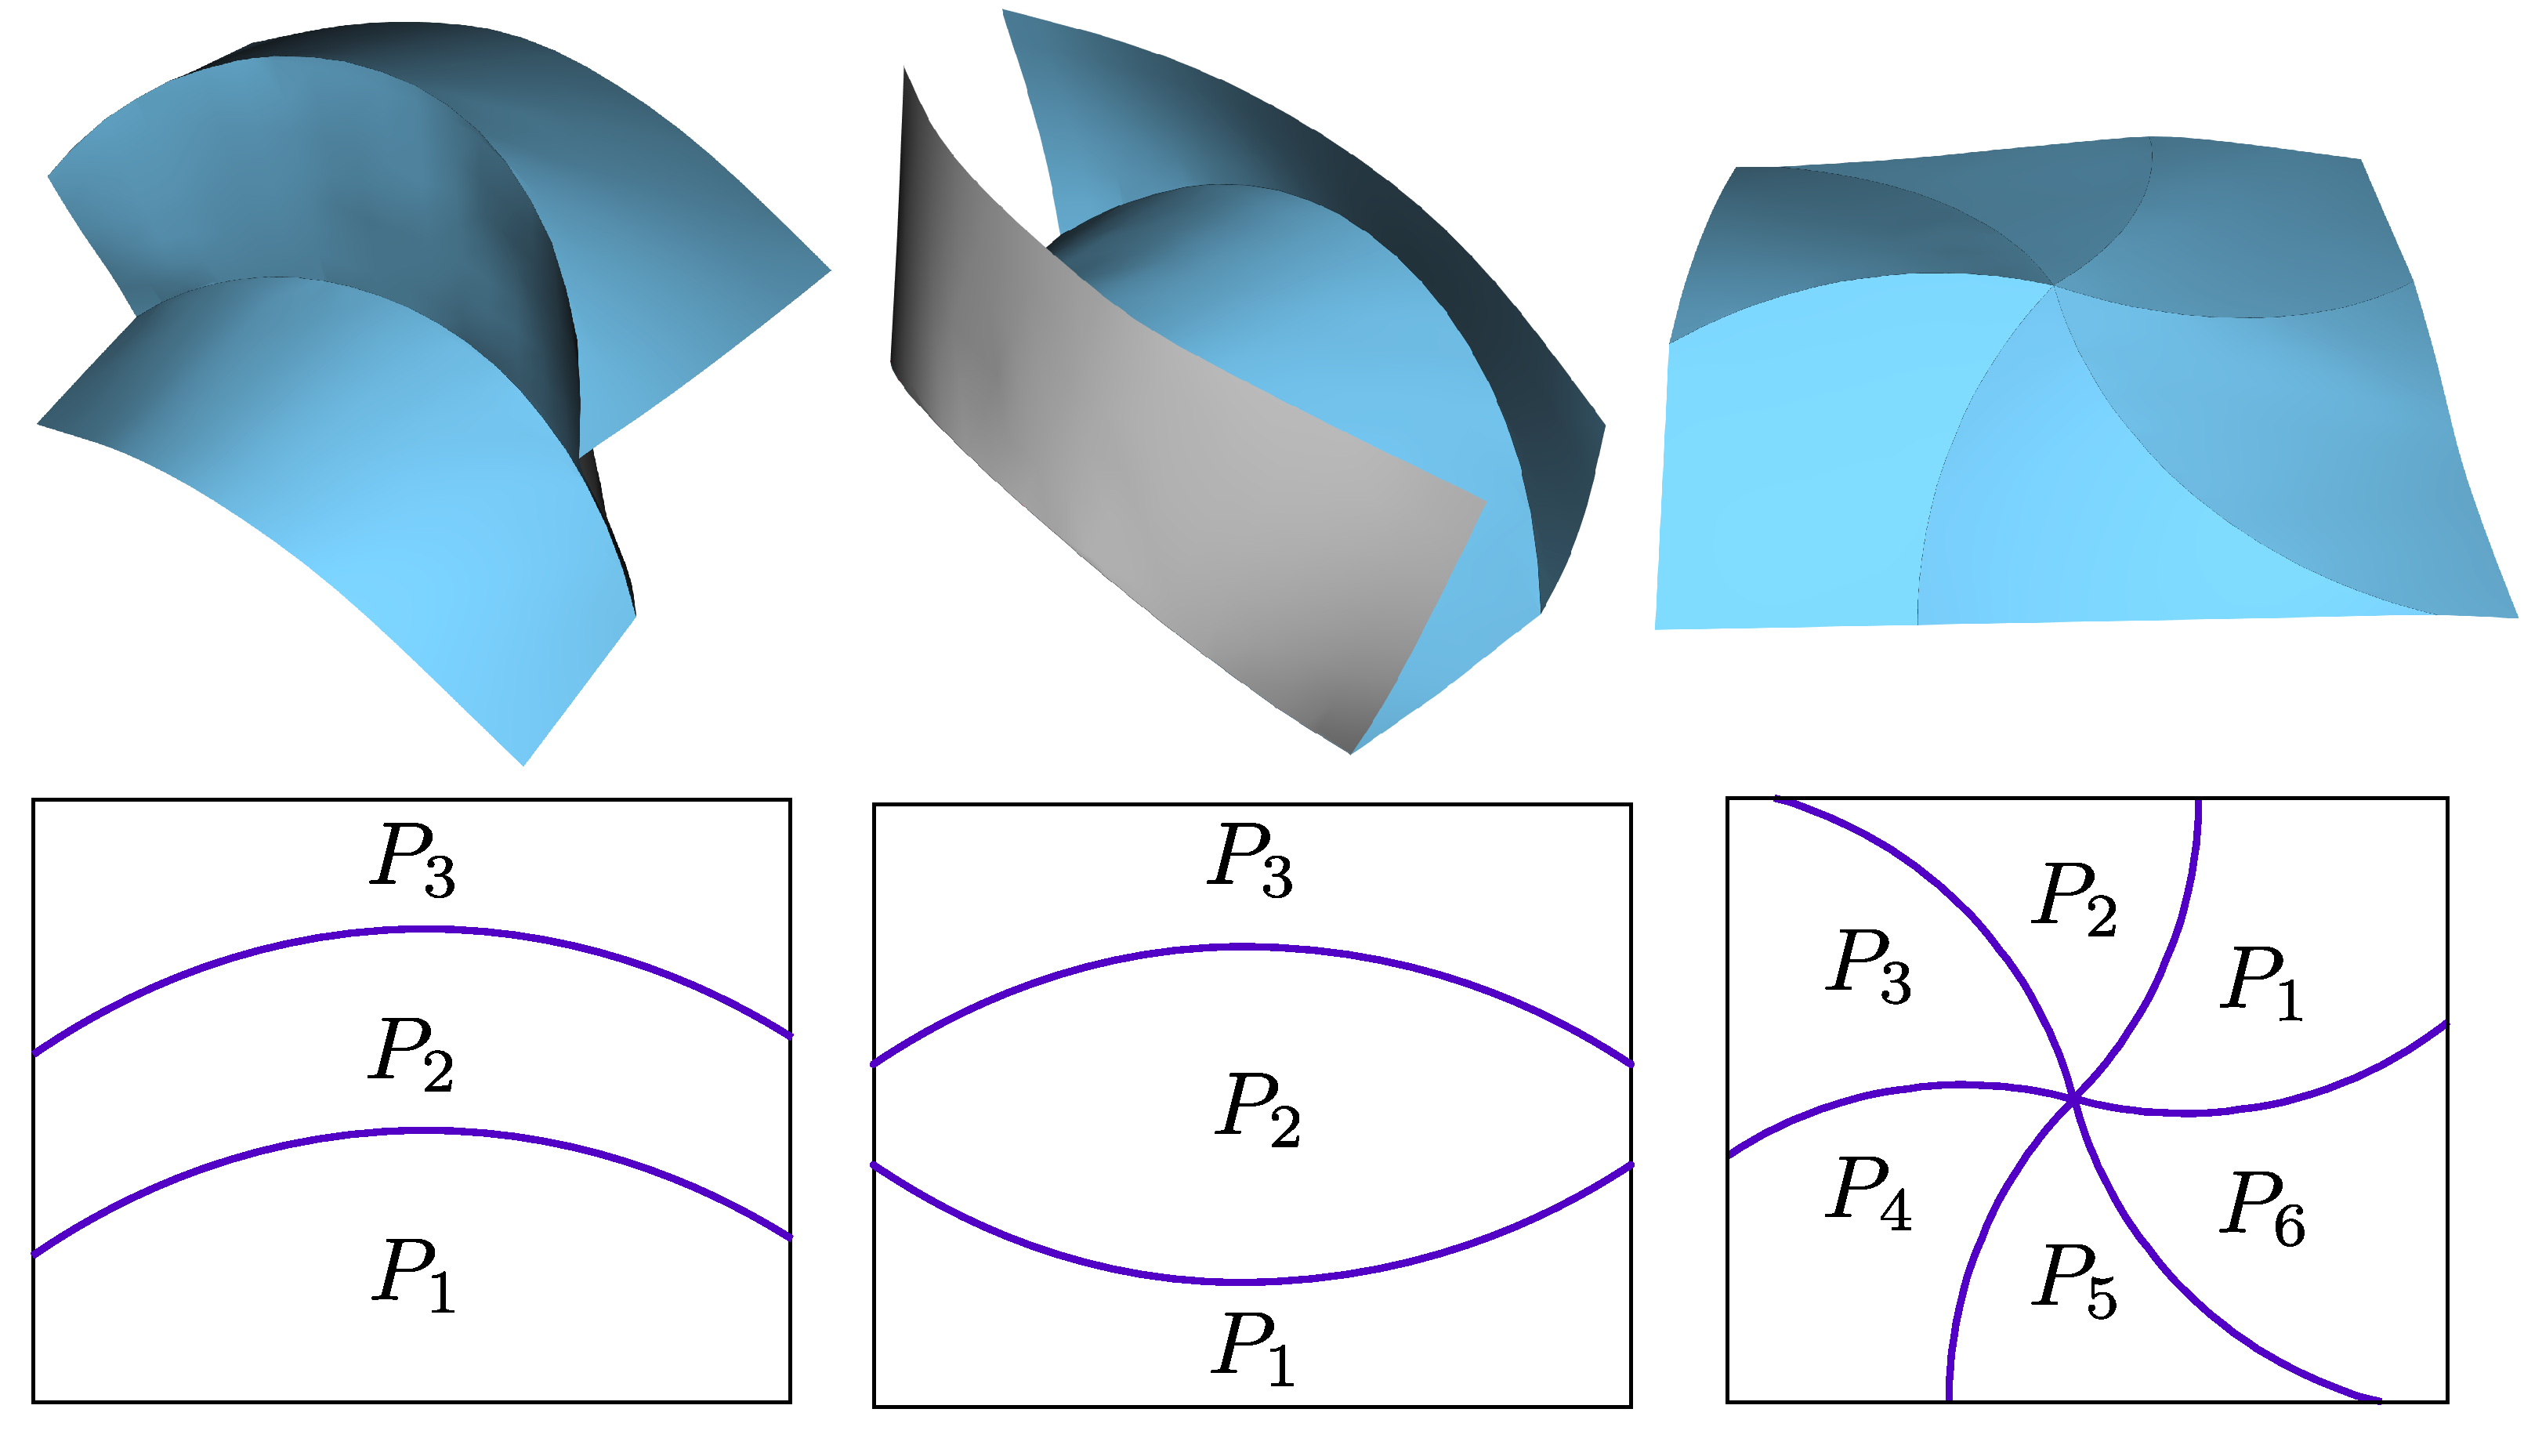
\includegraphics[width=0.7\linewidth]{figures/multiple_crease_patterns}
	\caption{Curved and straight crease patterns, decomposing a pattern into multiple components and intersecting at vertices.}
	\label{fig:multiple_crease_pattern}
\end{figure}

\section{Controlling the rulings} \label{sec:rulings}

\subsection{Controlling rulings along the curve} 
If the ruling angles of both surfaces along the crease are $\beta_1(t),\beta_2(t)$, measured by their angles with the tangents, then they satisfy the following \cite{more_on_paper,duncan_folded}:

\begin{equation}
\cot\beta_1(t) = \frac{\alpha'(t)-\tau(t)}{k(t)\sin(\alpha(t))},\cot\beta_2(t) = \frac{-\alpha'(t)-\tau(t)}{k(t)\sin(\alpha(t))}
\end{equation}
Which from here we can deduce (\cite{mathematical_omnibus,duncan_folded}):
\begin{equation} \label{cot_eq}
\begin{split}
\cot\beta_1(t) + \cot\beta_2(t) = \frac{-2\tau(t)}{k(t)\sin(\alpha(t))},\\
\cot\beta_1(t) - \cot\beta_2(t) = \frac{2\alpha'(t)}{k(t)\sin(\alpha(t))},
\end{split}	
\end{equation}
The authors of (\cite{mathematical_omnibus,duncan_folded}) identified two special cases, corresponding to when the above equations vanish. The first correspond to a planar curved fold, i.e. $\cot\beta_1(t) + \cot\beta_2(t) = \tau = 0$ which implies $\beta_1+\beta_2 = \pi$, meaning the rulings are continuation of each other on the flattened surface. In that case the two surfaces are just reflections of each other through the unique osculating plane of the curve (which doesn't change as $\tau = 0$). The second case corresponds to constant dihedral angle along the curve, i.e. $\cot\beta_1(t) - \cot\beta_2(t) = \alpha(t)' = 0$ which implies $\beta_1 = \beta_2$. These two cases coincide in the case $\beta_1 = \beta_2 = \frac{\pi}{2}$ (see \figref{fig:curved_different_rullings}).


\begin{figure} [h]
	\centering
	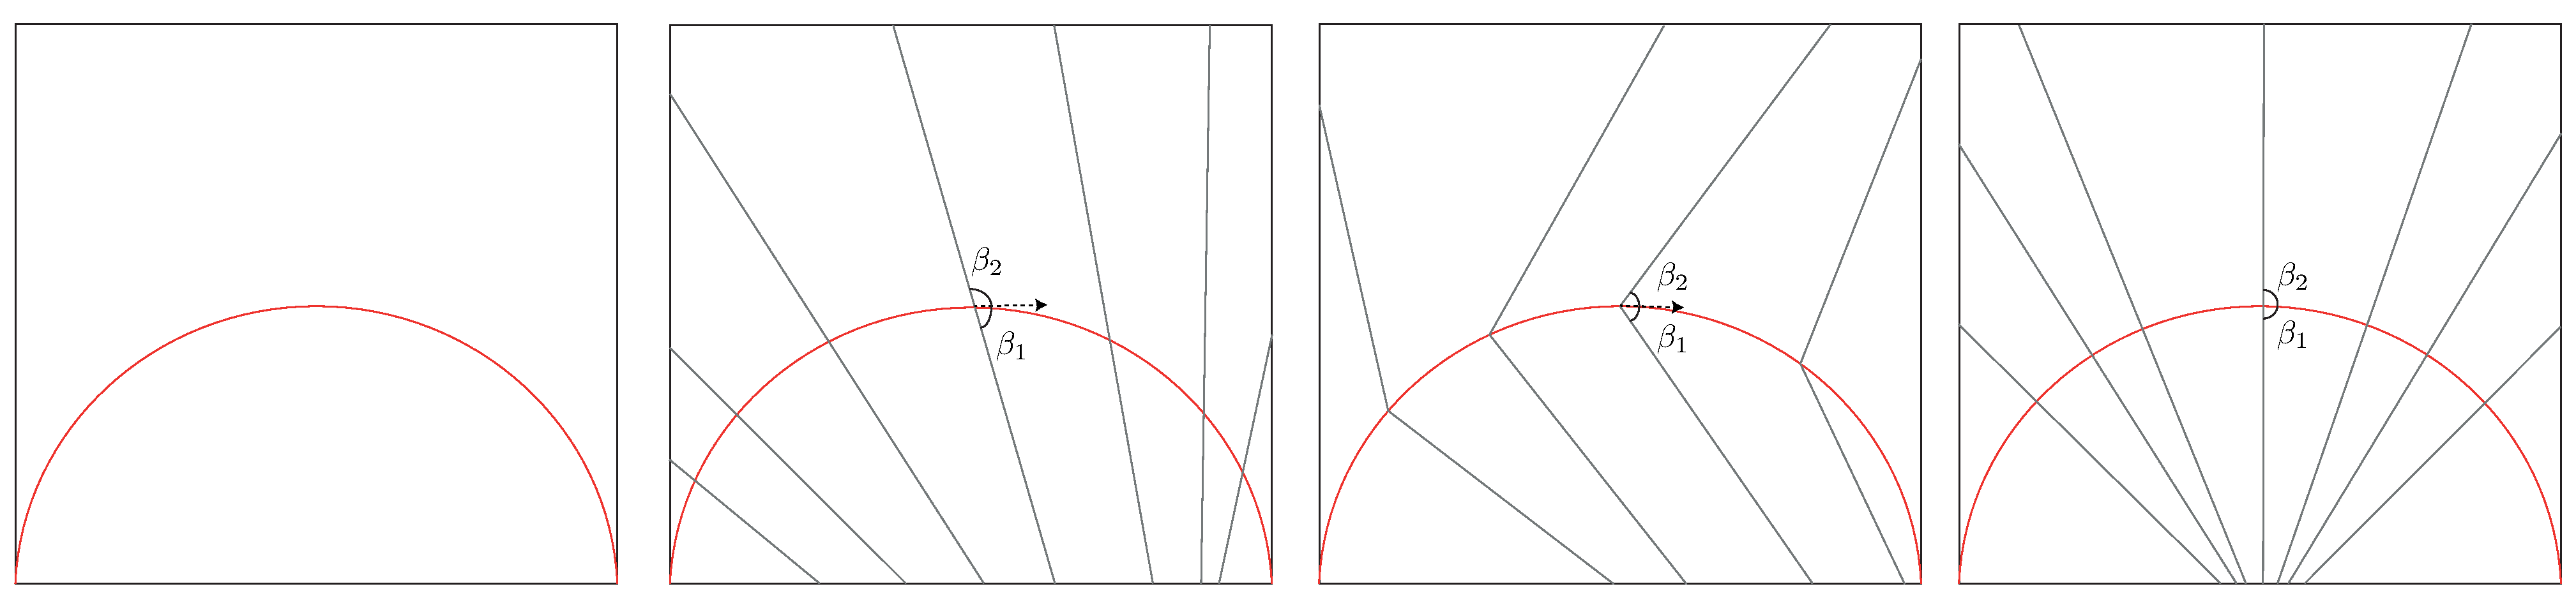
\includegraphics[width=\linewidth]{figures/curved_different_rullings}
	\caption{Different rulings patterns on a circular curved fold, displayed on the flattened configuration. From left to right: A circular curved fold pattern, a ruling pattern corresponding to $\beta_1(t)+\beta_2(t)=\pi$ (implying the curved fold is planar in 3D), a ruling pattern corresponding to $\beta_1(t)=\beta_2(t)$ (implying the dihedral angle between the tangent planes along the curve is constant) and a ruling pattern corresponding to both when $\beta_1(t)=\beta_2(t)=\frac{\pi}{2}$}
	\label{fig:curved_different_rullings}
\end{figure}

\subsection{Rulings objectives on DOG vertices}

\section{Applications} \label{sec:app}
\section{Conclusions and future work}
This paper is a first step towards unhindered freeform modeling of curved folded surfaces. Basing our models on DOGs \shortcite{rabi18} allows us to capture the full set of curved folded deformations, and our discretization in \secref{sec:folding} together with the folding algorithm in \secref{sec:implementation} allows us to steer the modeled deformations towards those that simultaneously fold and bend crease curves. Our deformation algorithm is able to model bending and folding of complicated crease patterns by merely using positional constraints, making it highly suited for exploration of new curved folded surfaces. We supply further optional objectives to constrain dihedral angles and mountain/valley assignment in \secref{sec:folding_angles_mountain_valley}, giving designers additional expressiveness. \\
Similar to other works on modeling DOGs \shortcite{rabi18,rabi2018shape}, the most obvious limitation of our algorithm is speed. Our optimization framework allows us to interactively model up to $2000$ vertices. We leave scaling of the optimization to future work, possibly by using a multigrid solver on the DOG grids. Throughout the design, we found that we lacked tools and objectives to enforce symmetry. In particular, we would like to look at folding of curved symmetric plane wallpappers and tessellations \cite{demaine_lens,mundilova2019mathematical}. Finally, we note that we model deformations of a given fixed input crease pattern. Optimizing and changing an input crease pattern, as done in origami modeling tools \cite{tachi2010freeform}, could offer new and exciting ways to discover and design curved folded surfaces. 

% Bibliography
\bibliographystyle{ACM-Reference-Format}
\bibliography{CurvedFoldedDogs}

\appendix


\end{document}